\newcommand{\comment}[1]{}

%\documentclass[a4paper,twocolumn,12pt]{article}

%\documentclass[a4wide,12pt]{report}

%\documentclass[a4wide,12pt]{article}
%\documentclass[informasjonssikkerhet]{gucmasterproject}
\documentclass[informationsecurity]{gucmasterproject}

%\usepackage{pslatex} %% Doesn't seem to work - i.e. convert .eps to .pdf
 
\usepackage[utf8]{inputenc}     % For utf8 encoded .tex files
%\usepackage[latin1]{inputenc}
\usepackage[norsk]{babel}     % For chapter headings etc.
%\usepackage[pdftex]{graphicx}           % For inclusion of graphics

%From http://math.uib.no/it/tips/
   %% For grafikk
    \usepackage{ifpdf}
    \ifpdf
      \usepackage[pdftex]{graphicx}
      \usepackage{epstopdf}
    \else
      \usepackage[dvips]{graphicx}
    \fi
    %% Her kan du putte dine vanlige pakker og definisjoner



%\usepackage[dvips]{hyperref}    % For cross references in pdf
\usepackage{hyperref}
\usepackage{mdwlist}
\usepackage{url}
\usepackage{here}

\def\UrlFont{\tt}

\begin{document}

\thesistitle{IMT5391 Service Design - NAV}
\thesisauthor{Engedal, J. Ø., Grimsgaard, C., Pedersen, K.}
\thesisdate{\gucmasterthesisdate}
\useyear{2014}
\makefrontpages % make the frontpages
%\thesistitlepage % make the ordinary titlepage


\comment{
Front page - including
"   HIG technical report front page including logos etc.
"   The text: "MSc project plan"
"   Title of project
"   Name of author and contact details
"   Date
"   Version

email address
"   MAIS students must include "NISlab" as their affiliation.
Date:22.10.2003

Structure of MSc thesis project plan
Gj�vik University College
}


\chapter*{Forord}

Dette er en delinnlevering den 22. mai. Rapporten vil være ufullstendig, minimalistisk og lite polert, men vil kunne gi foreleser mulighet til å gi gruppa tilbakemeldinger på arbeidet så langt.

\newpage

\begin{abstract}
Her vil det være et sammendrag av oppgaven. Det skriver vi til slutt.

\end{abstract}


\tableofcontents






\chapter{Dagens løsning hos NAV}
\section{Refleksjon rundt NAV}
\subsubsection{Hvor ligger problemet vedrørende alderspensjon?}
\begin{itemize}
\item For komplisert med tanke på regler
\item Lite konkret informasjon om hva man må kunne og vite om alderspensjon
\item Veldig få unge vet hvordan man faktisk sparer alderspensjon 
\item Alt for mye informasjon på sidene fører til liten interesse i å lese og lære seg hva alderspensjon er og hvordan det fungerer.
\item Informasjon om regler og annen informasjon man nødvendigvis ikke trenger, bør ikke være tilstede sammen med annen viktigere informasjon.
\item Ingen oppsummering fører til veldig kjedelig sider
\end{itemize}

\subsubsection{Forslag til forbedringer}
\begin{itemize}
\item Lage oppsummering av de viktigste emnene/sakene
\item Forenkle fremvisning av informasjon (runde bobler som på beta??)
\item Lage enkel grafikk som erstatter videoen om grisen
\item Dropdown/expand mulighet for sære/viktige/annen info
\end{itemize}



\section{Analyse av stakeholders}




\section{Personas}
\subsection{Thomas Larsen}
\textbf{Navn:} Thomas Larsen \\
\textbf{Alder:} 24 \\
\textbf{Yrke:} Elektriker \\
\textbf{Sivilstand:} Ugift \\
\textbf{Utdanning:} Yrkesfaglig med fagbrev \\
\textbf{Forhold til NAV mtp alderspensjon:} Lever i sin egen verden med lite kjennskap til hvordan alderspensjon fungerer og sin rolle i det. Stoler på arbeidsgiver. \\
\textbf{Teknisk kompetanse:} Gjennomsnittlige IT-kunnskaper. Har en iPad som brukes mest for underholdning.  \\
\textbf{Beskrivelse:} Thomas Larsen jobber i Elektriske A/S som holder til i Stavanger. Han leier en leilighet der han bor sammen med hunden sin. På fritiden liker han å spille fotball og går jevnlig på Viking-kamper sammen med kompiser. Han bruker iPhone 5 og iPad til å holde kontakt med venner via sosiale medier, samt til underholdning via enkle spill på iPad. Har en gammel Acer laptop som brukes veldig lite, der han bruker Mozilla Firefox som sin valgte nettleser. Har ingen tidligere erfaringer med NAV. Det eneste han vet om alderspensjon er at arbeidsgiver betaler inn en hvis prosentandel av utbetalt lønning. Tenker svært lite på alderspensjon siden han er såpass ung og ikke har trengt å tatt stilling til dette enda. \\
\textbf{Mål:} Ønsker seg mer informasjon om hvordan man tjener opp til alderspensjon.  \\
\textbf{Analyse:} Thomas klikker seg inn på NAV.no sine nettsider. Han leter umiddelbart etter tema alderspensjon og ved hjelp av den globale menyen, klikker han seg inn på alderspensjon. Her blir han umiddelbart litt forvirret, da han ikke vet hva som er relevant for sin egen situasjon.


\subsection{Gudrun Bekkehavn}
\textbf{Navn:} Gudrun Bekkehavn \\
\textbf{Alder:} 44 \\
\textbf{Yrke:} Lærer på barneskole \\
\textbf{Sivilstand:} Gift med Arne Bekkehavn \\
\textbf{Utdanning:} Lærer utdanning på høgskolenivå + et par fag som etterutdanning \\
\textbf{Forhold til NAV mtp alderspensjon:} Har god kontroll over sin alderspensjonsplan. Har hatt “veiledningsmøter” med NAV og fått god informasjon innenfor dette.  \\
\textbf{Teknisk kompetanse:} Det at hun er ansvarlig for IT-opplæringen ved skolen, gjør at hun har god kontroll på tekniske løsninger.  \\
\textbf{Beskrivelse:} Gudrun og Arne holder til i Fredrikstad i et stort hus. De har to barn, Jarle på 23 og Silje på 20. Gudrun er mye opptatt med sin lærerrolle og setter pris på fritiden hun har. Derfor liker hun å være effektiv i dagligdagse gjøremål.  Hun er ofte innom NAV på Din Side for å sjekke diverse informasjon og holde tritt på sin egen alderspensjonsplan.  \\
\textbf{Mål:} Ønsker å sjekke status på sin opptjente alderspensjon. 


\subsection{Pål Wolfgang}
\textbf{Navn:} Pål Wolfgang \\
\textbf{Alder:} 63 \\
\textbf{Yrke:} Kundebehandler ved DNB (20%) \\
\textbf{Sivilstand:} Gift med Mia Wolfgang \\
\textbf{Utdanning:} Økonomi og ledelse ved UiO \\
\textbf{Forhold til NAV mtp alderspensjon:} Er i ferd med å alderspensjonere seg og har dialog med NAV vedørende utbetaling og overgangen til aktiv alderspensjonisttilværelse. \\
\textbf{Beskrivelse:} Pål er en godt likt kundebehandler som er i ferd med å alderspensjonere seg. Han har nettopp flyttet inn i ny leilighet, sentralt i Oslo sentrum sammen med sin hustru. Han har gode IT-kunnskaper som han har lært seg via diverse kurs relevante til sin jobb som kundebehandler. Akkurat nå skal han bli alderspensjonist og gleder seg til å ta tidlig alderspensjon.  \\
\textbf{Mål:} Ønsker å gå av med alderspensjon og få sin første utbetaling.




\newpage
\section{Kundereise}

\begin{figure}[h!]
	\centering
	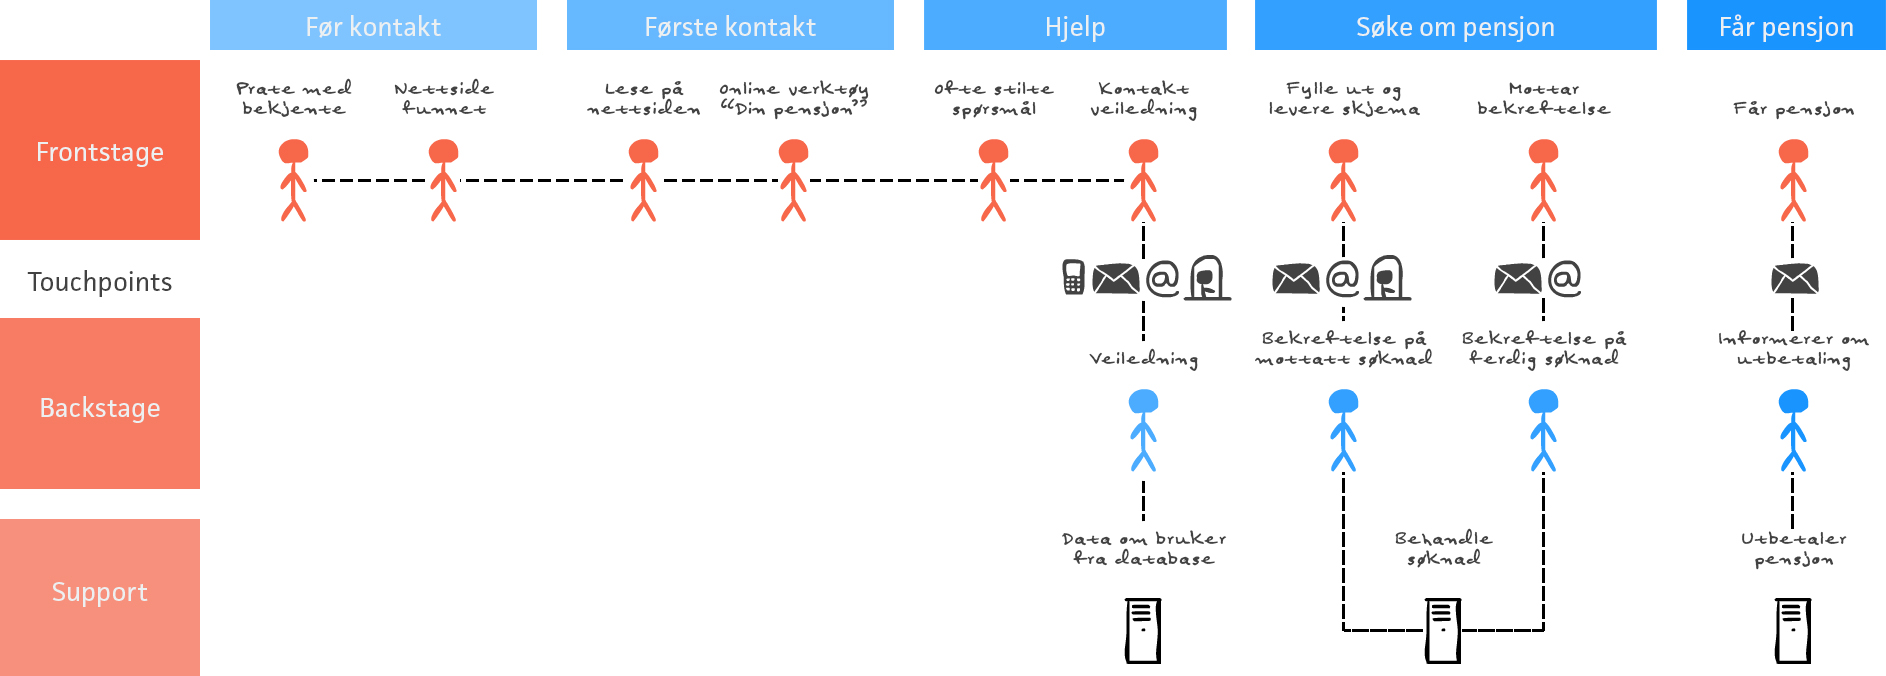
\includegraphics[width=59em, angle=270]{kundereise}
	\caption{Kundereisen visualisert.}
	\label{fig:kundereise}
\end{figure}

Her er en skriftlig beskrivelse av kundereisen.(1) betyr det som kalles frontstage. Dette er det brukeren gjør, ser og opplever. (2) står for backstage, som er det NAV gjør som brukeren ikke er spesielt oppmerksom på. Mellom (1) og (2) er det som kalles touchpoints; der brukeren møter NAV. Her nevner vi også på hvilken måte brukeren er i kontakt med NAV. (3) står for de hjelpelige prosessene, som f.eks. datasystemer, databaser osv.

\subsubsection{Før kontakt}
\begin{itemize}
\item (1) Prate med bekjente
\item (1) Nettside funnet
\end{itemize}

\subsubsection{Første kontakt}
\begin{itemize}
\item (1) Lese på nettsiden
\item (1) Online verktøy “Din alderspensjon”
\end{itemize}

\subsubsection{Hjelp}
\begin{itemize}
\item (1) Ofte stilte spørsmål
\item (1) Kontakter veiledning
	\begin{itemize}
	\item Telefon
	\item Fysisk
	\item Epost
	\item Post
	\end{itemize}
\item (2) Veileder
\item (3) Data om bruker fra database
\end{itemize}

\subsubsection{Søk om alderspensjon}
\begin{itemize}
\item (1) Fylle ut og levere skjema
	\begin{itemize}
	\item Post
	\item Fysisk
	\end{itemize}
\item (2) Bekreftelse på mottatt søknad
\item (3) Behandle søknad
\item (2) Bekreftelse på ferdig søknad
	\begin{itemize}
	\item Epost
	\item Post
	\end{itemize}
\end{itemize}

\subsubsection{Får utbetalt alderspensjon}
\begin{itemize}
\item (3) Utbetaler alderspensjon
\item (2) Informerer om utbetaling
	\begin{itemize}
	\item Post
	\end{itemize}
\item (1) Får alderspensjon
\end{itemize}




\chapter{Refleksjon}
Jacob Nilsen definerer brukskvalitet som
\begin{itemize}
\item Noe som er lett å lære, så nybegynnere raskt kan gå igang med arbeid
\item Effektivt, slik at ekspert brukere oppnår høy produktivitet
\item Enkelt å huske, slik at man kan begynne å arbeide raskt etter lang tids fravær
\item Behagelig å bruke, slik at man liker og bruke systemet
\item Minimerer sjansen for brukeren å gjøre katastrofale feil
\end{itemize}

Overføring fra et medium til et annet er ikke nødvendigvis bedre. Digitalisering av systemer som tidligere har brukt penn og papir fører ofte til økt grad av sosioteknisk kompleksitet. Dette kan bety f. eks at hvis det ligger en bunke papirer i en bestemt hylle, så vil enkelte arbeidsprosesser settes igang. Hvis man fjerner dette fysiske signalet, må man altså finne en måte å gjengi symbolikken i den digitale verden. Løsningen kan være å ha digitale bestemte postkasser til spesifikke formål, slik at brukerne av systemet enkelt kan fange opp meldinger. Hvis dette ikke gjøres, kan slike symboler blir glemt og systemet kan oppleve forsinkelser.

Ofte når man planlegger IKT systemer, går man ut ifra at alt er teknisk mulig. Dette skyldes i stor grad mangel på forståelse av IT og kompleksiteten ved store prosjekter. Man kan ikke bare kjøpe eller ta i bruk ny teknologi og forvente at alt vil bli bedre, ihvertfall i kortsiktig perspektiv. “Den største jobben ligger i prosessen med å ta  teknologien i bruk og tilpasse den  til organisasjonen, og med å tilpasse organisasjonen og arbeidsfordelingen og rutinene til det teknologien krever og muliggjør”. IKT: Et utfordrende redskap, KAP 9, Margunn Aanestad.

NAV har tilsvarende utfordringer med tanke på at det er forskjellige systemer som skal kunne komunisere med hverandre, både lokalt og nasjonalt. Derfor må man være ekstra grundig i forhånds arbeidet, der man ser på mer realistiske endringer, samt erkjenne, minimere og håndtere risiko. Eventuelle feil og problemer kan forplante seg og forårsake store forsinkelser, noe som er en svært  aktuel problemstilling når det gjelder NAV. 

Hva kan man gjøre med det? Det er viktig å forstå at det er flere aktører i spill når det gjelder så store og komplekse IKT systemer. God planlegging og realistiske målsetninger må være i fokus.




\chapter{Analyse av IT-systemer}
\section{Grunnleggende analyse}
En tradisjonell analyse av hvilke IT-systemer NAV bruker lar seg vanskelig gjennomføre, ettersom de benytter seg av 300 ulike IT-systemer fordelt på 12 hovedkategorier\footnote{http://sokelys.origo.no/-/bulletin/show/821802\_nav-under-lupen}. Sett bort fra spesifikke hensyn, kan man generalisere seg frem til at kompleksiteten i seg selv muligens er det mest kritiske problemet. Dersom dette ikke adresseres, vil selv store forbedringer i ett system være ubetydelige.

Agendaen vår i denne oppgaven er dog hverken spesifikk eller politisk, og selv om NAV er en kompleks entitet, vil nok alderspensjonssøkere bare forårsake systeminteraksjoner med en brøkdel av de aktuelle systemene. Vi har forsøkt å sende e-post til NAV for å undersøke hva slags spesifikke systemer de benytter seg av, men vi har ikke fått svar. Grunnen til at vi ikke møtte opp fysisk var rett og slett for å sette oss inn i et edge case-scenarie, som demonstrerer hvordan prosessen vil oppleves for en stum, enslig alderspensjonist med sosial angst, som derfor vil foretrekke å sende e-post.

Når det kommer til alderspensjon høres det egentlig ut som det meste fungerer fint. Prosessen oppleves som lettforståelig og ukomplisert, og ingen av besteforeldrene våre har problemer med NAVs alderspensjonstjenestedesign.

\section{CSCW-matrise}
\subsection{Samme sted, samme tid}
Dette er systemene som inngår i forbindelse med personlig oppmøte hos NAV. Selve backend-en kan antas å være den samme som ved andre sanntidsinteraksjoner over f.eks. telefon, som for eksempel registrering eller endring av personopplysninger. Alle slags databasesamhandlinger kan på en måte innordnes under alle de fire forskjellige punktene, ettersom de utgjør en sentral del av et hvert CSCW-scenarie.

Det vil sannsynligvis være de NAV-ansatte som blir nødt til å forholde seg til IT-systemer ved personlige oppmøter, ettersom noe av formålet ved å fysisk oppsøke NAV kan tenkes å være beleiligheten forbundet ved å slippe å måtte forholde seg til uforståelige IT-systemer eller forvirrende fagterminologi.

\subsection{Samme tid, forskjellig sted}
NAV tilbyr en rekke forskjellige muligheter for stedsuavhengig sanntidskommunikasjon. Dersom personlig oppmøte ikke er mulig eller er upraktisk, vil sannsynligvis telefonsamtaler være alderspensjonisters foretrukne løsning. Stedsuavhengigheten er en fordel for alderspensjonisten, men telefonmediet medfører visse vansker for den NAV-ansatte:
\begin{itemize}
\item Lydkvaliteten over telefon er dårlig.
\item alderspensjonister snakker ofte sykt utydelig.
\item Henvisninger til nettadresser eller skjemaer blir vanskelig, ettersom disse har kompliserte navnformater, og NAV-systemet er ganske komplekst for mannen i gata (og NAV-ansatte) å navigere.
\end{itemize}

NAVs chat-funksjonalitet er foreløpig en prøveordning for de som ønsker informasjon angående foreldrepenger, men det kan godt tenkes at NAV vil kunne tilby sanntidsekspertise innen deres andre tilbudsområder også. Merk våre ord - alderspensjonschat vil være en realitet innen 2020.

\subsection{Forskjellig tid, samme sted}
Dette kan muligens være en slags digital informasjonstavle i resepsjonen, eller annen informasjon som endres dynamisk, og skal aksesseres av de NAV-ansatte. Hvis man tolker begrepet bokstavelig, kan muligens en serie av personlige oppmøter være på forskjellig tid og samme sted.

\subsection{Forskjellig tid, forskjellig sted}
Steds- og tidsuavhengig elektronisk kommunikasjon vil hovedsaklig innebære e-post-kommunikasjon, eller NAV-spesifikke meldingssystemer. Sistnevnte har ikke vi tilgang til, og ingen av de vi spurte har uttrykt behov for å kommunisere med NAV på denne måten. E-postkorrespondansen vi selv opplevde var litt lite responsiv, men det kan tenkes at interne løsninger foretrekkes, og at de som faktisk er inne i systemet prioriteres.

\end{document}





IEEE computer society keywords
http://www.computer.org/portal/site/ieeecs/menuitem.c5efb9b8ade9096b8a9ca0108bcd45f3/index.jsp?&pName=ieeecs_level1&path=ieeecs/publications/author/keywords&file=ACMtaxonomy.xml&xsl=generic.xsl&
